\noindent
{
\color{red}
This chapter is intended to evaluate what you did.  The content is highly
topic-specific, but for many projects will have flavours of the following:

\begin{enumerate}
\item functional  testing, including analysis and explanation of failure
      cases,
\item behavioural testing, often including analysis of any results that
      draw some form of conclusion wrt. the aims and objectives,
      and
\item evaluation of options and decisions within the project, and/or a
      comparison with alternatives.
\end{enumerate}

\noindent
This chapter often acts to differentiate project quality: even if the work
completed is of a high technical quality, critical yet objective evaluation
and comparison of the outcomes is crucial.  In essence, the reader wants to
learn something, so the worst examples amount to simple statements of fact
(e.g., ``graph X shows the result is Y''); the best examples are analytical
and exploratory (e.g., ``graph X shows the result is Y, which means Z; this
contradicts [1], which may be because I use a different assumption'').  As
such, both positive {\em and} negative outcomes are valid {\em if} presented
in a suitable manner.
}

Using the automated testing suite the data harvested for the next section
was generated by averaging over 30 independant runs
each for 15000 generations. Each test was aimed at evolving circuitry
capable of 2-bit addition (and later 2-bit addition and subtraction). Evaluation
was performed as outlined in the previous chapter; for each of the 16 tests required
for 2-bit addition the binary representation of each number was made available
to the FPGA and after evaluating the circuitry 3 binary values are read off
the bottom of the grid, for each
correct bit the configuration scored 1 point. For 2-bit addition and weighted 2-bit
addition and subtraction the maximum score is 48.

\todo talk about the measurements - we measure the accuracy because it is
the metric we are trying to improve, not fitness

All experiments were conducted on a late 2013 15" Apple MacBook Pro with an
Intel Haswell Core i7 processor clocked at 2.3 GHz and 16GB of RAM.

\section{FPGA Simulator}
The main metric by which to judge the quality of the FPGA simulation is the
speed with which a configuration can be instantiated and evaluated.

\todo actually this

\section{GA Parameter Tuning}
All inital genetic algorithm parameters were set in accordance with
 \cite{10.1007/3-540-63173-9_61};
a population size of 50, with elitism, linear rank-based selection, the probability
of single point crossover occuring set to 0.7, and the expected mutations per
offspring set as 2.7. However the problem solved in \cite{10.1007/3-540-63173-9_61}
is dramatically different from the addition problem posed here so a great deal
of domain specific tuning is required.

\todo add more explicit parameters to figure
\begin{figure}
	\centering
	\begin{subfigure}[ht]{0.49\textwidth}
		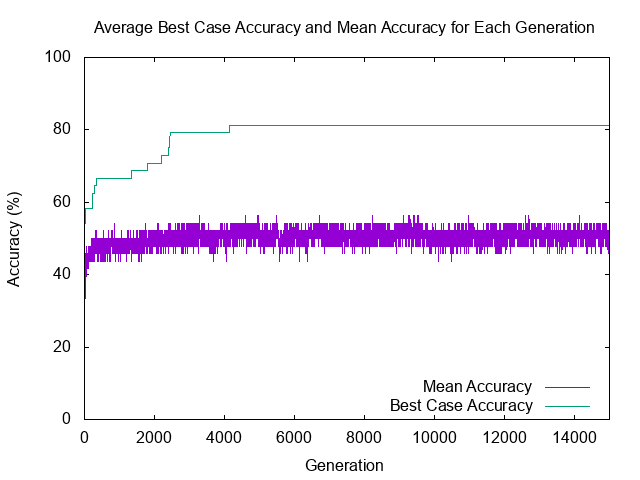
\includegraphics[width=\textwidth]{initial_test.png}
		\caption{}
		\label{fig:initial}
		\vspace{1em}
	\end{subfigure}
	~
	\begin{subfigure}[ht]{0.49\textwidth}
		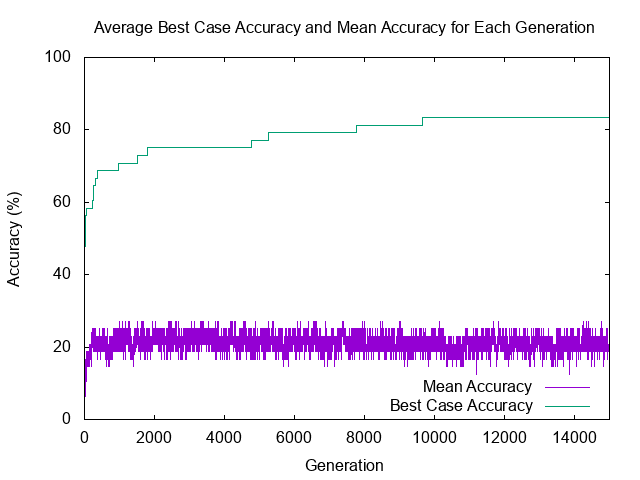
\includegraphics[width=\textwidth]{div_test.png}
		\caption{}
		\label{fig:initial_div}
		\vspace{1em}
	\end{subfigure}
	~
	\begin{subfigure}[ht]{\textwidth}
		\centering
		\begin{tabular}{ccccc}
			\toprule
			& \bfseries{Fitness Function} &
			\bfseries{Perfect Solutions (\%)} &
			\bfseries{Avg. Execution Time (s)} & \bfseries{Avg. Final Fitness}\\
			\midrule
			(a) & Simple & 0 & 235 & 39\\
			(b) & Multi-Objective & 0 & 267 & 40\\
			\bottomrule
		\end{tabular}
	\end{subfigure}

	\caption{Initial test results; (a) fitness over time when the parameters are
		initialised to \cite{10.1007/3-540-63173-9_61}, (b) fitness over time
		with an extended multi-objective fitness function incorporating a measure
		of diversity.}
\end{figure}

These parameters were evaluated and, as shown in Figure~\ref{fig:initial},
the results of these initial tests are
promising but show a great deal of room for improvement. Despite a healthy
initial improvement in fitness, this quickly reached a maximum score and
across the duration of the tests no evolutionary run was
capable of fomulating a perfect solution.
Visual inspection of this initial test as it ran highlighed a huge lack of
diversity in the population of solutions, every improvement in fitness was
an itterative change in the previous best case configuration. This occurs
when a solution improves beyond it's peers the boost to fertility leads to
it dominating the population. Often a dominating solution will be mostly
correct but due to wildly uneconomic uses of resources be completely incapabale
of evolving any further without dramatic backtracking. The user interface displays
the current average diversity; the distance from one individual to each other in the
population. Relatively early in execution when one member begins to dominate the
diversity plumits.

\todo include proof of plumiting diversity

The diversity in the population averaged (some value), which means that the average number
of different components between an individual and the rest of the population was
as little as 20. With an expected mutation rate of 2.7 this is
indicative of a population completely dominated by a single (potentially bloated)
solution as

\subsection{Improving Diversity}
Such evolutionary
dead ends were also faced by \cite{deJong:2001:RBP:2955239.2955241} who developed
a method of employing multi-objective fitness to encourage population diversity
and minimise waste in solutions. Using their multi-objective fitness function,
a linear combination of diversity and size, to improve the population diversity
and reduce the probability of bloated solutions could provide the evolutionary
pressure required to find a perfect solution.

A trial was conducted incorporating a diversity measurement weighted at 40\%
of the correctness weighting. The function does not include a measure of smallness
, as oversized solutions are not an immediate concern.

Figure~\ref{fig:initial_div} dipicts the results from this trail. Averaged across
all the runs, there was a slight increase in execution time acompanised by
a marginal improvement in the best case solution fitness
after 15000 generations. However, a larger number of generations was required
to match the correctness of the simpler fitness function. Despite predictions
to the contrary another symptom of
the more complex fitness function in this context is a reduced mean population fitness,
instead of easily beating 20 as happens in Figure~\ref{fig:initial},
\ref{fig:initial_div} maintains an
average of 10. This is due to a shift in evolutionary emphasis, in the new
scheme some individuals are given a large fitness due to their novelty alone
and therefore maintained despite their low fitness, which brings down the
average. This shift in emphasis also slows the
persuit of perfection; the intial trial in unencumbered with a fitness function
atempting to maintain diversity, and so aggresively persues improvements in
fitness due to a larger proportion of the population which are offspring of a
dominant individual. The slower intial gains in the second trial are indicative
of the smaller segment of the population actively working on the current best
configuration.

These findings disagree somewhat with \cite{deJong:2001:RBP:2955239.2955241},
who found vast improvements across the board when extending the fitness
function. However they did not experiment with population sizes as small
as presented here; unlike our population size of 50, DeJong et al. used
a population size of 1000. It could well be the case that
the population size is too small to facilitate a series of semi-idependently
evolving subpopulations.

To explore this further an experiment with 2 variables was conducted, varying
both the population size (50 and 500) and the incorporation (or not) of a
multi-objective fitness function combining diversity and correctness. A maximum
population size of 500 was used as a
size matching that of DeJong et al. would not feesable in the context as individual
runs would take in excess of 2 hours.

\todo add more explicit parameters to figure
\begin{figure}
	\centering
	\begin{subfigure}[ht]{0.49\textwidth}
		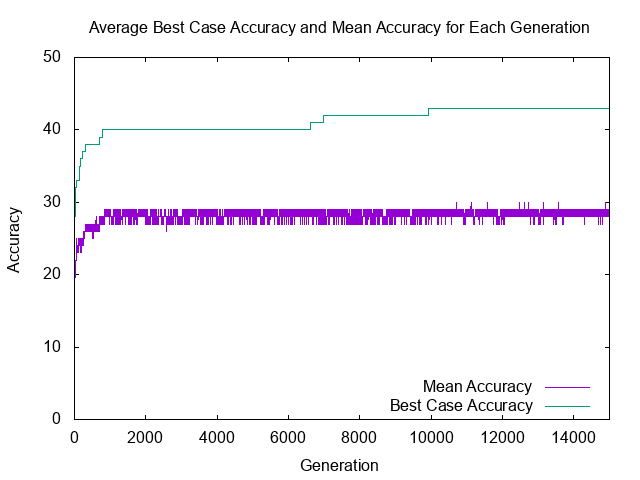
\includegraphics[width=\textwidth]{pop_500_no_div.png}
		\caption{}
		\label{fig:500_no_div}
		\vspace{1em}
	\end{subfigure}
	~
	\begin{subfigure}[ht]{0.49\textwidth}
		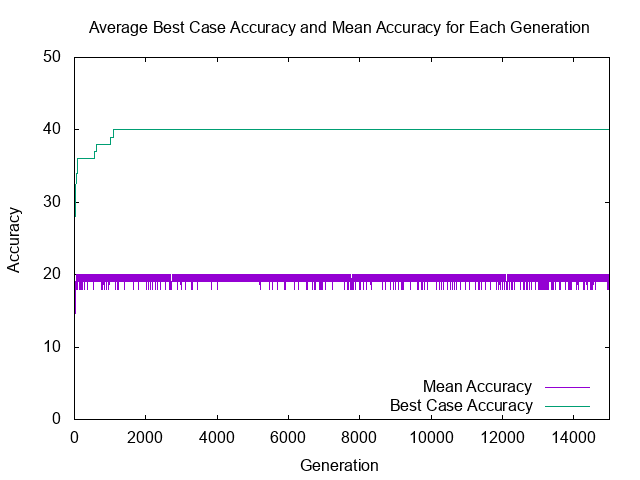
\includegraphics[width=\textwidth]{pop_500_div.png}
		\caption{}
		\label{fig:500_div}
		\vspace{1em}
	\end{subfigure}
	~
	\begin{subfigure}[ht]{\textwidth}
		\centering
		\begin{tabular}{ccccc}
			\toprule
			& \bfseries{Fitness Function} &
			\bfseries{Perfect Solutions (\%)} &
			\bfseries{Avg. Execution Time (s)} & \bfseries{Avg. Final Fitness}\\
			\midrule
			(a) & Simple & 0 & 2250 & 43\\
			(b) & Multi-Objective & 0 & 2857 & 40\\
			\bottomrule
		\end{tabular}
	\end{subfigure}

	\caption{Larger population diversity trail; (a) fitness over time with parameters
		initialised to \cite{10.1007/3-540-63173-9_61} but with a population of 500,
		(b) accuracy over time with an extended multi-objective fitness function and
	a population size of 500.}
	\label{fig:500}
\end{figure}

Figure~\ref{fig:500} contains the results from this experiment. The larger
population size with the simple fitness function (Figure~\ref{fig:500_no_div})
performed the best, the
streamlined persuit of accuracy combined with a larger pool of people to
draw from resulted in the best performance thus far. The extended function
(Figure~\ref{fig:500_div})
actually reduced the performance, again disagreeing with
\cite{deJong:2001:RBP:2955239.2955241}. This could be because
the larger population has natural diversity qualities, with a larger pool
a probabilistic procedure such as evolution naturally produces variance,
and the extended
function distracted too much from the persuit of accuracy. The hypothesis
that increasing the population size minimises the reduction in mean accuracy
does ring true. With the smaller population the extended fitness function resulted in
a mean accuracy of less than half the mean accuracy with the simpler fitness function,
whereas
with the a larger population the extended function's trail showed a mean accuracy of
more than
$2/3$rds that of the simpler one.

\todo fix these graphs (accuracy not fitness)

Despite the improved performance in Figure~\ref{fig:500_no_div} moving forward
further tuning will be performed on the parameters which produced Figure
~\ref{fig:initial_div}. The larger population size in the higher performer
produced an execution time which does not lend itself to exploration and
itterative improvement. Population size will, however, be futher explored on page
\todo reference.

\subsection{Mutation Rate}

\begin{figure}
	\centering
	\begin{subfigure}[ht]{0.49\textwidth}
		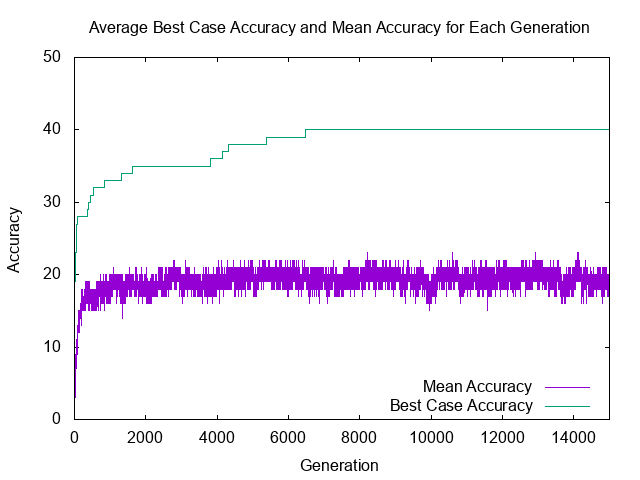
\includegraphics[width=\textwidth]{mut_1.png}
		\caption{}
		\vspace{1em}
	\end{subfigure}
	~
	\begin{subfigure}[ht]{0.49\textwidth}
		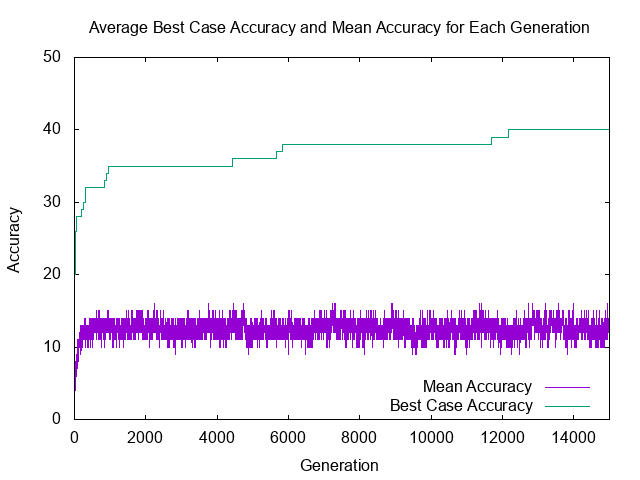
\includegraphics[width=\textwidth]{mut_2.png}
		\caption{}
		\label{fig:mut_2}
		\vspace{1em}
	\end{subfigure}
	~
	\begin{subfigure}[ht]{0.49\textwidth}
		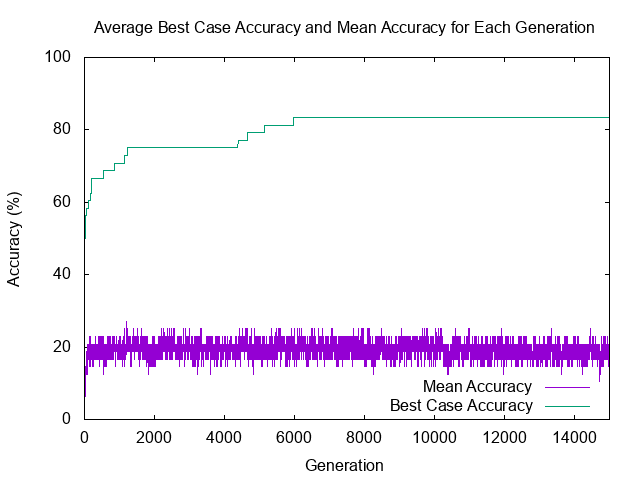
\includegraphics[width=\textwidth]{mut_3.png}
		\caption{}
		\label{fig:mut_3}
		\vspace{1em}
	\end{subfigure}
	~
	\begin{subfigure}[ht]{0.49\textwidth}
		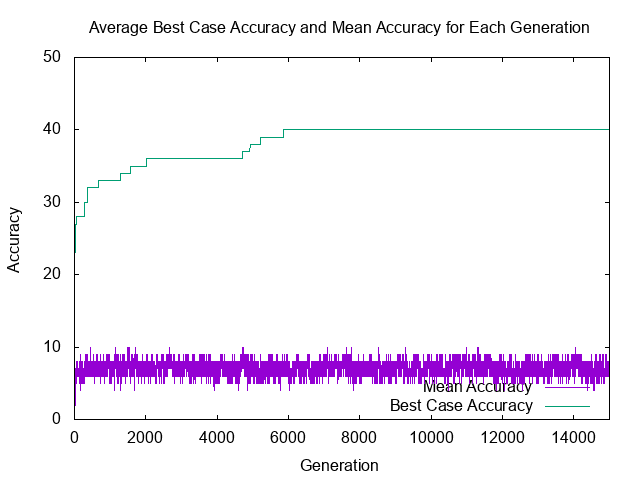
\includegraphics[width=\textwidth]{mut_4.png}
		\caption{}
		\vspace{1em}
	\end{subfigure}
	~
	\begin{subfigure}[ht]{\textwidth}
		\centering
		\begin{tabular}{ccccc}
			\toprule
			&\bfseries{Mutation Rate} &
			\bfseries{Perfect Solutions (\%)} &
			\bfseries{Avg. Execution Time (s)} & \bfseries{Avg. Final Fitness}\\
			\midrule
			(a) & 1 & 0 & 235 & 40 \\
			(b) & 2 & 0 & 235 & 40 \\
			(c) & 3 & 0 & 235 & 40 \\
			(d) & 4 & 0 & 235 & 40 \\
			\bottomrule
		\end{tabular}
	\end{subfigure}

	\caption{Mutation test results; (a) 1 expected mutation per individual,
		(b) 2 expected mutations per individual,
		(c) 3 expected mutations per individual,
		(d) 4 expected mutations per individual}
	\label{fig:mut}
\end{figure}

There are two main factors influencing the choice in mutation rate; the fragility
of solutions, and the space between viable individuals. If solutions to a problem are
inherrently fragile, as demonstrated in this case by Figure~\ref{fig:landscape}, then a high
mutation rate can regularly destroy working solutions and cause the system to
never rise above a fixed value. If the space between viable solutions is vast
a mutation rate which is too small will very rarely cause enough mutations to
span the ravine, yet alone create them in correct places. These two factors are
often at odds, no moreso than in this context where solutions are brittle and
sparse. Elitism is employed to reduce the impact of fragile solutions by ensuring
the best case solution is never lost, and the inclusion of the extended diversity
fitness function encourages individuals to drift across ravines rather than have
to make the journey in a single step. Therefore the impact of shifting the
fitness function is unclear.

The experiments conducted in Figure~\ref{fig:mut} mostly agree with the findings
in \cite{10.1007/3-540-63173-9_61}, however a slight performance increase in the
best case individual is
demonstrated when shifting the mutation rate from 2.7 (Figure~\ref{fig:initial_div})
to 3 (Figure~\ref{fig:mut_3}). The drastic reduction in the speed with which
the best case individual is evolved occuring with a mutation rate of 2
(Figure~\ref{fig:mut_2}) is unexpected. This result could be due to the underlying
topography of the solution landscape; viable solutions are rarely 2 changes apart,
and are more frequently distanced at 1, 3, or 4 changes. This would explain this
marginal reduction in speed. Note the continuous decrease in population mean accuracy
as the mutation rate is increased, the reasons are twofold; firstly, a higher mutation
rate is more likely to induce a change in an accuracy-critical component of the
solution. Secondly, with an extended fitness function maintaining solutions for
novel value alone, the more aggresive mutation rate is more likely to cast members of the
population into even further unexplored corners of the fitness landscape giving them
an even higher diversity score (and therefore improving their fitness) and these rarely have a high
accuracy score.

Because of the results demonstrated by Figure~\ref{fig:mut_3}, namely slighly
improved best-case evolution (at the cost of population accuracy), an expected
mutation rate of 3 has been chosen. This was selected over the mutation rate 1
as the higher population accuracy is a symptom of a more localised less varied
population which is cultivated by a gentler mutation rate.

\subsection{Selection Mechanisms}
The most popular selection methods in evolvable hardware by some margin are
ranks selection and tournament selection. Thus far we have been using linear
rank selection (mirroring \cite{10.1007/3-540-63173-9_61}). Here the use
of a variable skewed rank selection is emplyed to place higher evolutionary pressure
on the better performing individuals. The variable controlling the linearity
of the selection function can be set such that the probability of selection
grows quadratically rather than linearly as you move up the rankings. To this
end experiments setting this value to 0 (a quadratic function with no linear
component), 0.25, 0.5, 0.75, and 1
(completely linear) will highlight any impact this has on the system.

Along with this variation an experiment comparing current best
selection with tournament selection of varying sizes 10 (1/5th the population
size) upto 40 (4/5ths the population size). The smaller tournament size
will discriminate less against lower performing individuals, and the
larger the tournament the fewer poorly performing configurations will
be selected for the next generation.

\begin{figure}
	\begin{minipage}{\textwidth}
	\centering
	\begin{subfigure}[ht]{0.32\textwidth}
		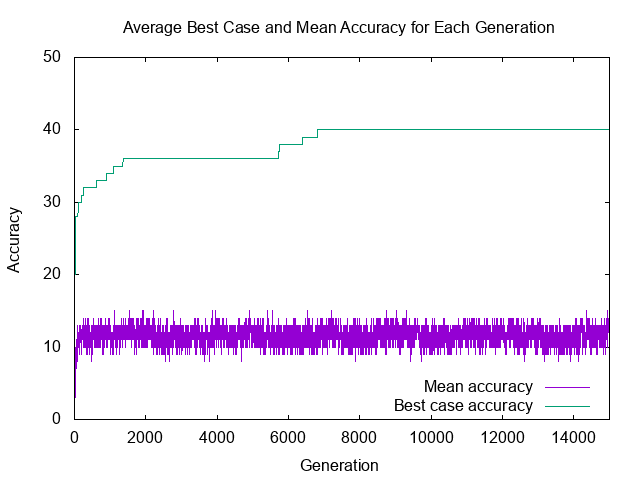
\includegraphics[width=\textwidth]{skew_0.png}
		\caption{}
		\label{fig:skew_0}
		\vspace{1em}
	\end{subfigure}
	~
	\begin{subfigure}[ht]{0.32\textwidth}
		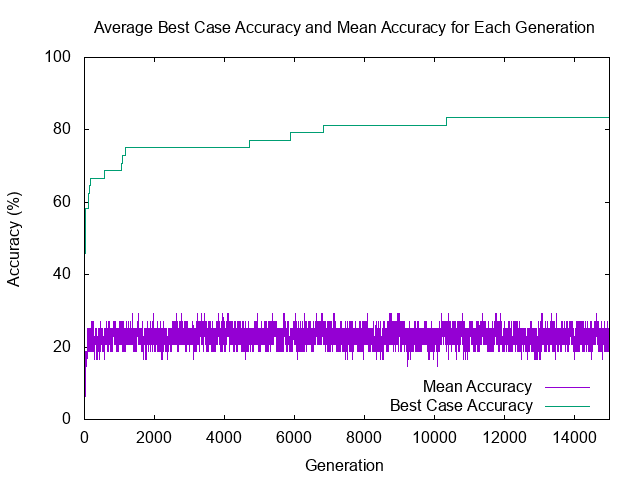
\includegraphics[width=\textwidth]{skew_point5.png}
		\caption{}
		\label{fig:skew_point5}
		\vspace{1em}
	\end{subfigure}
	~
	\begin{subfigure}[ht]{0.32\textwidth}
		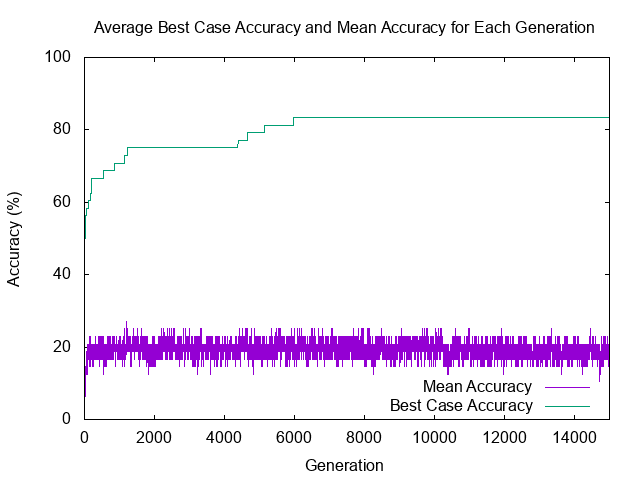
\includegraphics[width=\textwidth]{mut_3.png}
		\caption{}
		\label{fig:skew_1}
		\vspace{1em}
	\end{subfigure}
	~
	\begin{subfigure}[ht]{0.32\textwidth}
		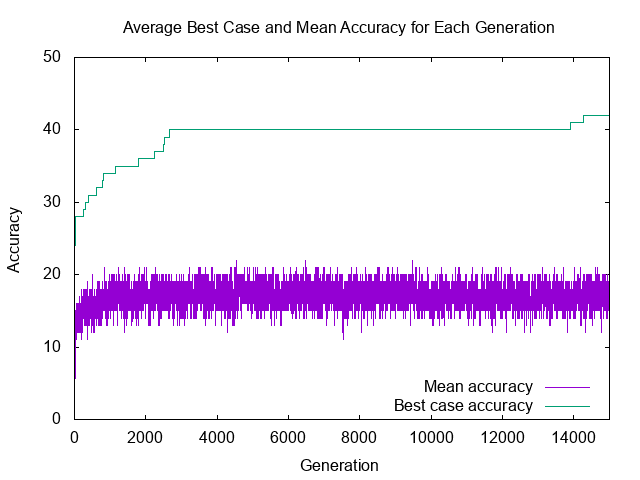
\includegraphics[width=\textwidth]{tour_10.png}
		\caption{}
		\label{fig:tour_10}
		\vspace{1em}
	\end{subfigure}
	~
	\begin{subfigure}[ht]{0.32\textwidth}
		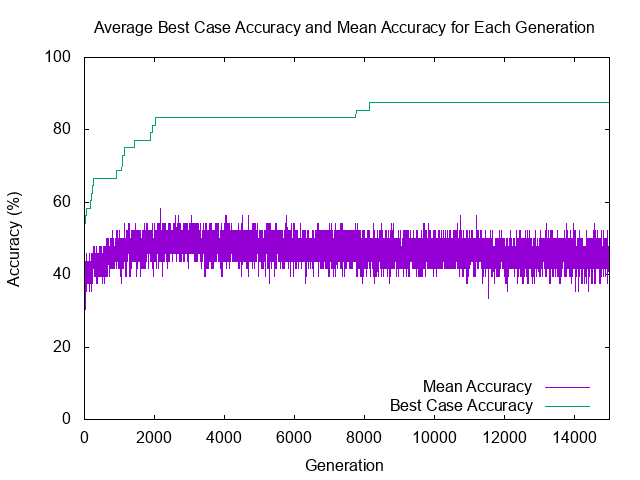
\includegraphics[width=\textwidth]{tour_20.png}
		\caption{}
		\label{fig:tour_20}
		\vspace{1em}
	\end{subfigure}
	~
	\begin{subfigure}[ht]{0.32\textwidth}
		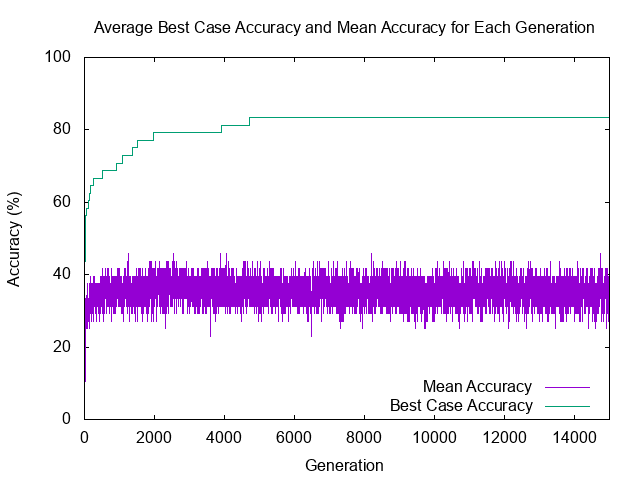
\includegraphics[width=\textwidth]{tour_30.png}
		\caption{}
		\label{fig:tour_30}
		\vspace{1em}
	\end{subfigure}
	~
	\begin{subfigure}[ht]{0.32\textwidth}
		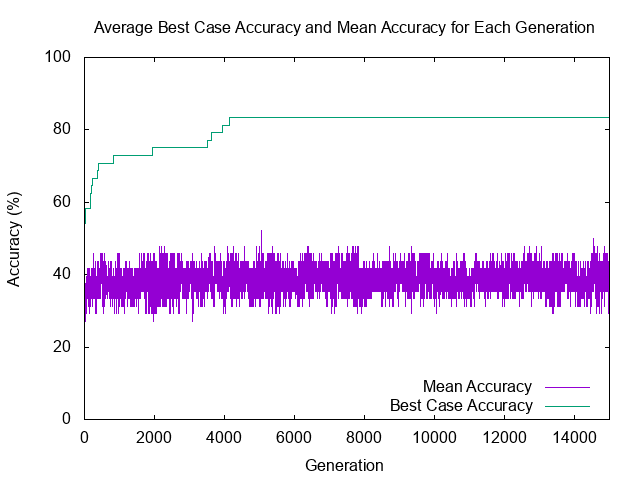
\includegraphics[width=\textwidth]{tour_40.png}
		\caption{}
		\label{fig:tour_40}
		\vspace{1em}
	\end{subfigure}
	~
	\begin{subfigure}[ht]{\textwidth}
		\centering
		\begin{tabular}{ccccc}
			\toprule
			& \bfseries{Selection Method} &
			\bfseries{Perfect Solutions (\%)} &
			\bfseries{Avg. Execution Time (s)} & \bfseries{Avg. Final Fitness}\\
			\midrule
			REDO THIS (a) & Rank (Skew 0.0) & 0 & 415 & 38 \\
			(b) & Rank (Skew 0.5) & 0 & 415 & 40 \\
			(c) & Rank (Skew 1.0) & 0 & 363 & 40 \\
			(d) & Tournament (Size 10) & 0 & 264 & 42 \\
			(e) & Tournament (Size 20) & 13 & 231 & 42 \\
			(f) & Tournament (Size 30) & 3 & 260 & 40 \\
			(g) & Tournament (Size 40) & 0 & 244 & 40 \\
			\bottomrule
		\end{tabular}
	\end{subfigure}

	\caption[Selection method test results; (a)(b)(c)
	rank based
	selection with skew 0.0, 0.5, and 1.0 respectively
	, (d)(e)(f)(g) using tournament selection with tournament
	size 10, 20, 30, and 40 respectively]{Selection method test results; (a)(b)(c)\footnote[1]{(c) duplicated from Figure~\ref{fig:mut_3} for better direct
	visual comparison} rank based
	selection with skew 0.0, 0.5, and 1.0 respectively
	, (d)(e)(f)(g) using tournament selection with tournament
	size 10, 20, 30, and 40 respectively}
	\label{fig:select}
\end{minipage}
\end{figure}

The more aggresive discrimination against members of the population due to the
variable skew is clear in Figure~\ref{fig:select}. The population under a more
aggressive selection mechanism (Figure~\ref{fig:skew_0}) persue the
maximum accuracy somewhat quicker than the more linear rank selections
(Figure~\ref{skew_point5} and Figure~\ref{skew_1}).

\subsection{Crossover}
Crossover works well in this context, the nature of the mapping between genotype
and phenotype means any crossover can provide benifits to both mating pairs and
inject some much needed diversity into the ecosystem. Six different trial runs
were execuited, each at a different crossover probability rate; 0, 0.25, 0.5,
0.75, and 1. Crossover points only occur between bytes, never inside them; so
when genetic material is transplanted it is always clean and operation is
consistent before and after.

\subsection{Elitism}
With a reduced mutation rate the effect of elitism is diminished. As the probability
of a correct solution being mutated away and broken is reduced. Elitism by it's very
nature leads to less diverse populations, but it is often a necessity in evolvable
hardware to stop systems regressing. Binary arithmatic is especially fragile.

\subsection{Tuning Population Size}
With the desire to cultivate a diverse population at the forefront of the parameter
selection reasoning enlarging the population would improve the spread of solutions,
and allow the evolutionary pressure on diversity to simultaneously mature and
develop a bredth of solutions.
Obviously increasing the size of the population has objective benifits in a statistical
sense by casting the net wider, more individuals means a higher chance to stumble
accross the correct solution.
But, this has diminishing returns; due to the diversity measurement incorporated into
the fitness function the evalutation time grows with $O(n^2)$ complexity with the
population size.

The increased population size from the experiments with a multi-objective
fitness function could be beyond the point of diminishing returns. To explore this
further trials varying the population size to explore how execution time and
genetic algorithm performance is affected.

\subsection{Tuning Diversity}

\subsection{Size}

\subsection{Coevolution}

In a coevolutionary system there a host of problems that can disturb the gentle
ballance between host and parasite, (red queen etc)

Thus far, in all experiments after a certain amount of time the average population
fitness reaches a plateau and all improvements seem to come from the highest performing
individual(s) with little impact in the overall population. This behaviour is indicative
of a disengaged population
\todo Talk about all the coevolutionary problems from Bullocks paper

By now we have a relatively well performing evolutionary hardware system,
tailored directly for the binary arithmatic problem. With this we can explore
a range of uses within the domain of dynamic problems.

\subsection{Evolved 2-bit addition hardware}
Talk about all the cool stuff, success rate etc analyise the given circuit
beyond simple correctness.

\begin{figure}
	\centering
	
\includegraphics[width=0.45\textwidth]{evolved_adder.png}
	\caption{Can add}
\end{figure}

\section{Fault tollerance}

The dynamic problem with the largest immediate impact is arguably that of
a system experiencing faulty behaviour.
With a tuned genetic algorithm, exploration into the capacity to dyanmically
adapt the configuration in the face of such a changed or changing problem provides
the oportunity to thoroughly test fault recovery and mitigation strategies.

Using the fault simulation framework built into the FPGA simulation a series
of targeted or randomly generated faults will be introduced to an in-progress
genetic algorithm.

\subsection{Simple Fault Recovery}
By preloading the genetic algorithm with a hand designed 2-bit adder and then
simulating a highly targeted critical fault withing the function of a CLB insight
can be gained into the capcity of evolvable hardware to act as a fault recovery
system in itself and provide a reliable method of recalibration should a device
experience a fault which would otherwise render it useless.

\begin{figure}
	\centering
	\begin{subfigure}[ht]{0.45\textwidth}
		
\includegraphics[width=\textwidth]{perfect_adder.png}
	\end{subfigure}
	~
	\begin{subfigure}[ht]{0.45\textwidth}
		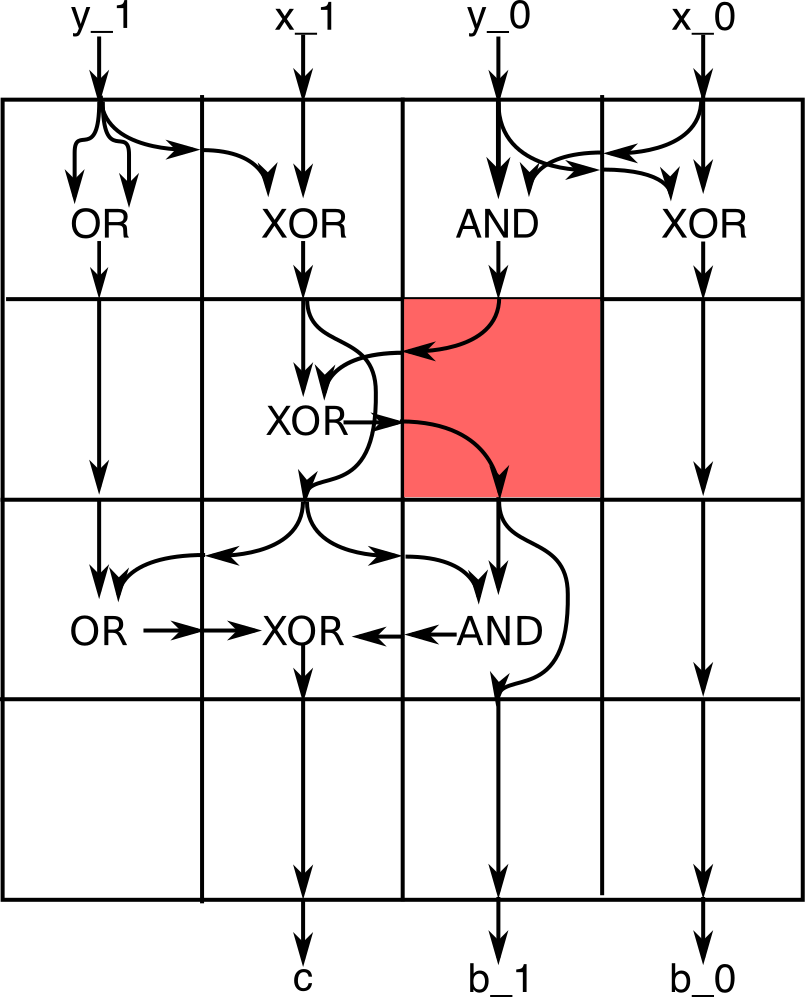
\includegraphics[width=\textwidth]{perfect_adder_fault.png}
	\end{subfigure}
	\caption{Fault recovery}
\end{figure}

\subsection{``Sticky" Fault Mitigation}
Evolutionary hardware can be used to recover from otherwise devastating faults. In the example below the outputs of the operation F within the CLB marked in red were clamped to a value representing an “undefined output”. Starting with the ideal configuration on the left and activating the fault, the genetic algorithm recognised the current solution as suboptimal and generated the configuration on the right.

Simulating a sticky fault by activating and deactivating a fault every 500 generations results in the fitness graph above on the right. When the fault is activated it has an adverse affect on fitness, but a solution is found which works when the fault is both active and inactive.

Sticky faults improve diversity and therefore improve training, maybe

Different from normal Fault tollerance - this is the sticky fault model to find a design okay for all, instead the evolution happens when the fault is detected to recover

\section{Dynamic problem optimisation}
By introducing subtraction as a problem alongside addition, the relative weightings of a correct answer for each problem can be varied to explore dynamically changing problems. In the graph below the genetic algorithm starts with a perfect ADDer and 100\% of the fitness weighting assigned to correct ADDs, every 200 generations this shifts by 10\% towards SUBs.

\section{Scaling}
In an effort to improve how an evolvable hardware system scales observing
how the dynamics of a coevolutionary system vary as the number of parasites
fluctuates could indicate a potential mechanism to reduce the number of
test cases required per evaluation and therefore improve evaluation time.

Evaluating the execution time and correctness of the solutions generated
by the genetic algorithm as we reduce the size of the parasite should
quantify the feesability of this idea.

Scafolding vs non-scafolding, coevolution to improve scalability of finess evaulation (tests grow expontentiallly as input bits increase)

\section{Physical Implimentation}
Using quantum physical phenomina

\section{Evolution good}
better than bruteforce
mention things set out to do and address challenges

\section{Evolution bad}
Intermittent leap from primordeal soup
